% TODO:

% Write ``Liquid-vapor interface'' section A.

% Look up question-mark references (citations).

\documentclass[letterpaper,twocolumn,amsmath,amssymb,jcp,10pt,aip]{revtex4-1}
\usepackage{graphicx}% Include figure files
\usepackage{dcolumn}% Align table columns on decimal point
\usepackage{bm}% bold math
\usepackage{color}

\newcommand{\red}[1]{{\bf \color{red} #1}}
\newcommand{\blue}[1]{{\bf \color{blue} #1}}
\newcommand{\green}[1]{{\bf \color{green} #1}}
\newcommand{\rr}{\textbf{r}}
\newcommand{\refnote}{\red{[ref]}}

\newcommand{\fixme}[1]{\red{[#1]}}

%\newcommand{\derivation}[1]{#1} % Use this to show all derivations in detail
\newcommand{\derivation}[1]{} % Use this for nice pegagogical paper...

% needsworklater is used to annotate bits that need work, but that we
% can postpone for a while.
\newcommand{\needsworklater}[1]{\emph{[#1]}}
% needsworknow is intended to prioritize stuff that needs fixing.
\newcommand{\needsworknow}[1]{\textcolor{red}{[\emph{#1}]}}

\begin{document}
\title{Using Fundamental Measure Theory to Treat the Correlation
  Function of the Inhomogeneous Hard-Sphere Fluid}

\author{Jeff Schulte}
\author{Patrick Kreitzburg}
\author{Chris Haglund}
\author{David Roundy}
\affiliation{Department of Physics, Oregon State University, Corvallis, OR 97331}


%%%%%%%%%%%%%%%%%%%%%%%%%%%%%%%%%%%%%%%%%%%%%%%%%%%%%%%%%%%%
\begin{abstract}
  We investigate the value of the correlation function of an
  inhomogeneous hard-sphere fluid at contact.  This
  quantity plays a critical role in Statistical Associating Fluid
  Theory (SAFT), which is the basis of a number of recently developed classical
  density functionals.  We define two averaged values for the
  correlation function at contact, and derive formulas for each of
  them from the White Bear version of the Fundamental Measure Theory
  functional~\cite{roth2002whitebear}, based on an assumption of
  thermodynamic consistency. We test these formulas, as well as two
  existing formulas~\cite{yu2002fmt-dft-inhomogeneous-associating,
    gross2009density} against Monte Carlo simulations, and find
  excellent agreement between the Monte Carlo data and one of our
  averaged correlation functions.
\end{abstract}

\maketitle

%%%%%%%%%%%%%%%%%%%%%%%%%%%%%%%%%%%%%%%%%%%%%%%%%%%%%%%%%%%%
\section{Introduction}

% The following are papers that use a SAFT-based classical DFT with at
% least some of the terms purely local
\newcommand\saftlocaldft{felipe2001examination, gloor2002saft,%
  gloor2004accurate, clark2006developing, gloor2007prediction,%
  kahl2008modified, gross2009density}
% The following are papers that use a SAFT-based classical DFT with
% all the terms that should be non-local being non-local.
\newcommand\saftnonlocaldft{yu2002fmt-dft-inhomogeneous-associating,%
  fu2005vapor-liquid-dft,bryk2006density}

There has been considerable recent interest in using Statistical
Associating Fluid Theory (SAFT) to construct classical density
functionals to describe associating
fluids\cite{\saftlocaldft,\saftnonlocaldft}.  This approach has been
successful in qualitatively describing the dependence of surface
tension on temperature.
%
%% Unfortunately, most of these constructed
%% functionals\cite{\saftlocaldft} cannot be used to study arbitrary
%% inhomogeneous density distributions, because they use local density
%% approximations that are only valid for densities that vary slowly over
%% molecular length scales.
%
A key input to SAFT-based functionals is the correlation function
evaluated at contact.

%% Constructing a classical density functional based on SAFT involves
%% rewriting each term in the free energy as a functional of an
%% inhomogeneous density.  The SAFT free energy consists of four terms:
%% \begin{align}
%%   A_\textit{SAFT} &= A_\textit{ideal} + A_\textit{HS} + A_\textit{chain} + A_\textit{disp} + A_\textit{assoc}
%% \end{align}
%% where $A_\textit{ideal}$ is the ideal-gas free energy, $A_\textit{HS}$
%% is the excess free energy of a hard-sphere fluid, $A_\textit{chain}$
%% is the free energy of formation for polymeric fluids,
%% $A_\textit{disp}$ is the dispersion contribution to the free energy,
%% and $A_\textit{assoc}$ is the free energy contribution from
%% \emph{association}, which is to say, hydrogen bonding.  

The chain and association terms in the SAFT free energy are of
particular interest for this paper, since each requires as input the
contact value of the correlation function.  The chain term describes
the chain formation energy in polymeric fluids, while the association
term describes the effects of hydrogen bonding, both of which can be
large.
%
Yu and Wu introduced in 2002 a functional for the association term of
the free energy, which included a functional for the contact value of
the correlation function (described in
Section~\ref{sec:yuwu})\cite{yu2002fmt-dft-inhomogeneous-associating},
which has subsequently been used in the development of other
SAFT-based functionals\cite{fu2005vapor-liquid-dft, bryk2006density}.
%% Each of these terms has some dependence on the
%% inhomogeneity in the density.  The ideal gas is purely local, and in
%% fact must be the only purely local term in the free energy in order
%% for the functional to satisfy the contact-value theorem.  The
%% hard-sphere contribution contribution to the free energy has been
%% thoroughly studied, and is well approximated by the White Bear version
%% of the Fundamental-Measure Theory (FMT)
%% functional\cite{roth2002whitebear}.
Two functionals for the chain contribution have recently been
introduced\cite{bryk2006density, gross2009density}, one which uses the
correlation function of Yu and Wu\cite{bryk2006density}, while the
other introduces a new approximation for the contact value of the
correlation function (described in
Section~\ref{sec:gross})\cite{gross2009density}.
%% The dispersion term is long-range and thus has significant
%% dependence on the density distribution, but because its relatively
%% weak position dependence, is amenable to mean-field approximations.
Given these different approaches, it seems valuable to examine this
property of the hard-sphere fluid through direct simulation, in order
to establish the advantages and disadvantages of each approach.

Although these recent works have introduced approximate functionals
for the contact value of the correlation
function\cite{yu2002fmt-dft-inhomogeneous-associating,
  gross2009density}, there has not been a study that specifically
addresses the correlation function at contact of an inhomogeneous
hard-sphere fluid.
%
In this paper we introduce two definitions for the locally averaged
correlation function of an inhomogeneous system.
%
%% The first is more symmetric (which we call the $S$ case), while the
%% second involves a sphere-centered, assymetrical interpretation (the
%% $A$ case).
%
Given these definitions, we will present a thermodynamic derivation
for each correlation functions from the free energy functional.  We
will then discuss the correlation functions of Yu and Wu of Gross, and
will end by comparing all four approximations with Monte-Carlo
simulations of the hard-sphere fluid at a variety of hard-wall
surfaces.


\section{Correlation function with inhomogeneity}

We define our terms using the two-particle density
$n^{(2)}(\rr_1,\rr_2)$, which gives the probability per unit volume
squared of finding one particle at position $\rr_1$ and the other at
position $\rr_2$.  The pair correlation function is defined by
\begin{align}
  g(\rr_1,\rr_2) &\equiv \frac{n^{(2)}(\rr_1,\rr_2)}{n(\rr_1)n(\rr_2)}
\end{align}
In a homogeneous fluid, the pair correlation only depends on the
distance $|\rr_1-\rr_2|$ and can be expressed as a function of a
single variable. The contact value is this correlation evaluated at a distance of the
diameter $\sigma$.  It is desirable for reasons of efficiency to limit CDFT
functionals to one-center convolutions, which leads us to seek a
simplified expression for the contact value of the correlation
function---which is the same as the contact value of the cavity
correlation function for hard spheres.
In a system with an inhomogeneous density, we seek a \emph{local}
value for $g_\sigma$.  There are two reasonable options for defining
such a local function: a symmetric formulation (which we refer to as $S$) and an
asymmetric formulation (which we refer to as $A$).

For the symmetric $S$ case, the correlation function at contact is
given by:
\begin{align}
  g^S_\sigma(\rr) &= \frac{1}{n_0(\rr)^2}\int n^{(2)}(\rr - \rr', \rr
  + \rr')
  \frac{\delta(\sigma/2 -|\rr'|)}{\pi\sigma^2}d\rr' \label{eq:gS}
\end{align}
where density $n_0$ is one of the fundamental measures of Fundamental
Measure Theory (FMT), and is ideal for treating touching spheres, as
illustrated in Figure~\ref{fig:n0}.
\begin{align}
  n_0(\rr) &= \int n(\rr')\frac{\delta(\sigma/2 -|\rr-\rr'|)}{\pi\sigma^2} d\rr'
\end{align}
This functional gives a value averaged over all spheres that touch at
the position $\rr$.

\begin{figure}
\includegraphics[width=5cm]{figs/n0}
\caption{Set of hard spheres that included in $n_0(\mathbf{r})$, which
  consist of those which just touch the point $\mathbf{r}$.}
\label{fig:n0}
\end{figure}

In contrast, the asymmetrically averaged $A$ correlation function is
given by
\begin{align}
  g^A_\sigma(\rr) &= \frac{1}{n(\rr)n_A(\rr)}
  \int n^{(2)}(\rr, \rr + \rr')
  \frac{\delta(\sigma -|\rr'|)}{4\pi\sigma^2}d\rr' \label{eq:gA}
\end{align}
where the density $n_A(\rr)$ is similar to $n_0$, but measures the
density of spheres that are touching a sphere that is located at
point $\rr$.
\begin{align}
  n_A(\rr) &= \int n(\rr')
  \frac{\delta(\sigma -|\rr-\rr'|)}{4\pi\sigma^2} d\rr' \label{eq:nA}
\end{align}
Thus $g_\sigma^A$ corresponds to an average of the two-particle
density over spheres touching a sphere that is located at the
position~$\rr$.

%% In the process of defining these two averaged correlation functions,
%% we also defined two averaged densities, $n_0(\rr)$ and $n_A(\rr)$,
%% which are the density of spheres available to be in
%% contact.  In the homogeneous limit, $n_0 = n_A = n$.  It is an
%% open question, which of these averages will be more useful in any
%% particular functional.  Suffice to say, either average is a
%% \emph{possible} way to convert a function that is defined for a
%% homogeneous system to a functional that is applicable to inhomogeneous
%% systems.

%% Yu and Wu introduce an approximation for
%% $g^S$\cite{yu2002fmt-dft-inhomogeneous-associating}, which we will
%% discus in Section~\ref{sec:yuwu}.  Gross introduced an
%% approximation for $g^A$\cite{gross2009density}, which we will
%% introduce in Section~\ref{sec:gross}.  We will also introduce our own
%% approximations for both $g^A$ and $g^S$ which are based on the
%% assumption of thermodynamic consistency within FMT, in
%% Sections~\ref{sec:g-S} and~\ref{sec:g-A}.  We will report on the accuracy of
%% these approximations by comparing with Monte Carlo simulations of the
%% inhomogeneous hard-sphere fluid.  We will focus on the contact
%% densities, rather than the correlation function itself, because these
%% are simpler, and because they are the quantity that you want to
%% ``average''.  i.e. if you were to average $g$ itself, you'd want to
%% weight that average based on the density, which would mean averaging
%% $n^{(2)}$.


%% \subsection{Association free energy of SAFT}

%% \fixme{Integrate the following equations into this section...}
%% \begin{align}
%%   \frac{A_\textit{chain}}{kT} &= -(m-1) n \left(\ln\left(n g_\sigma \right)-1\right)
%% \end{align}
%% \begin{align}
%%   \frac{A_\textit{assoc}}{kT} &= \sum_i n \left(\ln X_i - \frac12 X_i + \frac12\right) \\
%%   X_i &= \frac{1}{1 + \sum_j n g_\sigma X_j\kappa_{ij} \left(e^{\beta \epsilon_{ij}}-1\right)}
%% \end{align}

%% \newcommand\epsilonassoc{\ensuremath{\varepsilon_\textit{AB}}}
%% \newcommand\kappaassoc{\ensuremath{\kappa_\textit{AB}}}
\newcommand\ncontact{\ensuremath{n_\textit{contact}}}

%% The free energy term in Statistical Associating Fluid Teory (SAFT)
%% from which it derives its name is the association term, which accounts
%% for hydrogen bonding.  Hydrogen bonds are modeled as attractive
%% patches (``association sites'') on the surface of hard spheres.  These
%% sites represent protons or electron lone pairs, and have an attractive
%% energy $\epsilonassoc$ when two molecules are oriented such that the
%% proton of one overlaps with the lone pair of the other.  The volume
%% over which this interaction occurs is $\kappaassoc$, giving the
%% association term in the free energy has two empirical parameters fit
%% to experimental data.

%% The association free energy per unit volume has the form
%% \begin{align}
%%   f_\text{assoc} &= k_BT n\sum_A 
%%                   \left(\ln X^A - \frac{X^A}{2} + \frac12\right)
%% \end{align}
%% where the summation is over the association sites, and $X^A$ is the
%% fraction of association sites \emph{not} hydrogen-bonded.  The
%% fractions $X^A$ are determined by the self-consistent equations
%% \begin{align}
%%   X^A &= \frac{1}
%%   {1 + \sum_B n X^B \Delta^{AB}}\label{eq:X}
%%   \\
%%   \Delta^{AB} &= g(\sigma) \kappaassoc\left( e^{\epsilonassoc/kT} -
%%   1 \right)\label{eq:delta}
%% \end{align}
%% where $g(\sigma)$ is the correlation function evaluated at contact.
%% The product of density with correlation function evaluated at contact
%% gives the contact density, when we combine Equations~\ref{eq:X} and
%% \ref{eq:delta}:
%% \begin{align}
%%   X^A &= \frac{1}
%%   {1 + \sum_B \ncontact\kappaassoc X^B\left( e^{\epsilonassoc/kT} -
%%   1 \right)}
%% \end{align}
%% where the product $\ncontact\kappaassoc$ is the expected number of
%% molecules present in the association volume in the absence of the
%% association interaction.  In the SAFT-VR
%% model\cite{gil-villegas-1997-SAFT-VR}, this contact density is found
%% by adding a perturbative correction to the contact value for a hard
%% sphere fluid.

\subsection*{Fundamental-Measure Theory}

We use the White Bear version of the Fundamental-Measure Theory~(FMT)
functional~\cite{roth2002whitebear}, which describes the excess free
energy of a hard-sphere fluid.  The White Bear functional reduces to
the Carnahan-Starling equation of state for homogeneous systems.  It
is written as an integral over all space of a local function of a set
of ``fundamental measures'' $n_\alpha(\rr)$, each of which is written
as a one-center convolution of the density.  The White Bear free
energy is thus
\begin{equation}
A_\textit{HS}[n] = k_B T \int \left(\Phi_1(\rr) + \Phi_2(\rr) + \Phi_3(\rr)\right) d\rr \; ,
\end{equation}
with integrands
\begin{align}
\Phi_1 &= -n_0 \ln\left( 1 - n_3\right)\\
\Phi_2 &= \frac{n_1 n_2 - \mathbf{n}_{V1} \cdot\mathbf{n}_{V2}}{1-n_3} \\
\Phi_3 &= (n_2^3 - 3 n_2 \mathbf{n}_{V2} \cdot \mathbf{n}_{V2}) \frac{
  n_3 + (1-n_3)^2 \ln(1-n_3)
}{
  36\pi n_3^2\left( 1 - n_3 \right)^2
} ,
\end{align}
using the fundamental measures
\begin{align}
  n_3(\rr) &= \int n(\rr') \Theta(\sigma/2 -\left|\rr - \rr'\right|)
  d\rr' \label{eq:FMn3} \\
  n_2(\rr) &= \int n(\rr') \delta(\sigma/2 -\left|\rr - \rr'\right|) d\rr' \\
  \mathbf{n}_{2V}(\rr) &= \int n(\rr') \delta(\sigma/2 -\left|\rr - \rr'\right|) \frac{\rr-\rr'}{|\rr-\rr'|}d\rr'
\end{align}
\begin{align}
  \mathbf{n}_{V1} = \frac{\mathbf{n}_{V2}}{2\pi \sigma}, \quad
  n_1 &= \frac{n_2}{2\pi \sigma} , \quad
  n_0 = \frac{n_2}{\pi \sigma^2} \label{eq:FMrest}
\end{align}


\section{Theoretical Approaches}

\subsection{Homogeneous limit}

In order to motivate our derivation of the correlation function at
contact for the \emph{inhomogeneous} hard-sphere fluid, we begin by
deriving the well-known formula for $g_\sigma$ for the
\emph{homogeneous} fluid that comes from the Carnahan-Starling free
energy.  The contact value of the correlation function density can be
found by using the contact-value theorem, which states that the
pressure on any hard surface is determined by the density at contact:
\begin{align}
  p &= k_BT n_\textit{contact} \\
  &= k_BT n g_\sigma
\end{align}
Since we are interested in the correlation function at the surface of
the hard spheres, all we need compute is the pressure on that surface,
and we'll have our answer.  The pressure on a hard sphere can be
readily computed from the dependence of the Carnahan-Starling free
energy on hard sphere radius.
\begin{align}
  A_{HS} &= Nk_BT \frac{4\eta - 3\eta^2}{(1-\eta)^2}
\end{align}
where $\eta \equiv \frac{\pi}{6} \sigma^3 n$ is the filling fraction.
We can thus readily compute the derivative of free energy with respect
to hard-sphere diameter:
\begin{align}
  \frac{dA_{HS}}{d\sigma} &= \frac{dA_{HS}}{d\eta} \frac{d\eta}{d\sigma} \\
  &= Nk_BT \frac{4 - 2\eta}{(1-\eta)^3} \frac{3 \eta}{\sigma} \label{eq:dAhsdR}
\end{align}
This derivative gives us half the force on \emph{all} the hard
spheres---since we're changing all their radii at once.  To compute
the pressure on the spheres, we just need to divide by half the total
area, which means dividing by $N 8\pi \sigma^2$, since the relevant
area is the area over which the molecules can make contact.
\begin{align}
  p_\sigma &= \frac{1}{N 8\pi \sigma^2} \frac{dA_{HS}}{d\sigma} \\
  &= k_BT n \frac{1 - \frac{\eta}2}{(1-\eta)^3}
\end{align}
Using the contact-value theorem, we can thus find the well-known
correlation function evaluated at contact.
\begin{align}
  g_\sigma &= \frac{1 - \frac{\eta}2}{(1-\eta)^3} \label{eq:cs-g}
\end{align}
Extending this derivation to the inhomogeneous fluid requires that we
find the pressure felt by the surface of particular spheres.


\subsection{Asymmetrically averaged correlation function}\label{sec:g-A}

We will begin our derivation of the locally averaged correlation
function with the asymmetric definition of $g_\sigma^A(\rr)$ given in
Equation~\ref{eq:gA}, which is averaged over contacts in which one of
the two spheres is located at position~$\rr$.  This correlation
function is related to the contact density averaged over the surface
of a sphere located at $\rr$, and can thus be determined by finding
the pressure on that sphere.  We find this pressure from the change in
free energy changes resulting from an infinitesimal expansion of any
spheres located at position~$\rr$.  From this pressure, we derive a
formula for the correlation function $g_\sigma^A(\rr)$ as was done in
the previous section:
\begin{align}
  p_\sigma(\mathbf{r}) &= \frac{1}{n(\rr) 2\pi \sigma^2} \frac{\delta
    A_{HS}}{\delta \sigma(\mathbf{r})} \label{eq:p_{HS}^A}\\
%  \ncontact(\rr) &= \frac{1}{n(\rr) k_BT 2\pi \sigma^2} \frac{\delta
%    A_{HS}}{\delta \sigma(\mathbf{r})} \\
  g_\sigma^A(\rr)% &= \frac{\ncontact(\rr)}{n_A(\rr)} \\
  &= \frac{1}{n(\rr) n_A(\rr)}\frac{1}{ k_BT 2\pi \sigma^2} \frac{\delta
    A_{HS}}{\delta \sigma(\mathbf{r})} \label{eq:g-A-exact}
\end{align}
Details of evaluating the functional derivative in
Equation~\ref{eq:g-A-exact} using FMT are given in
Appendix~\ref{appendix:g-A}.  The equation for $g_\sigma^A$ requires
finding convolutions of local derivatives of the free energy, making
this formulation computationally somewhat more expensive than the free
energy itself.

\derivation{
  \end{widetext}
}

\subsection{Symmetrically averaged correlation function}\label{sec:g-S}

We now address the symmetrically averaged correlation function, which
is defined in Equation~\ref{eq:gS}.  This corresponds to the
correlation function averaged for spheres \emph{touching at a given
  point}.  In this case, we conceptually would like to evaluate the
pressure felt by the surface of spheres where that surface is located
at point~$\rr$.  We can approximate this value by assuming that this
pressure will be simply related to the free energy density at
point~$\rr$.  Through math similar to the previous derivations, this
leads to the expression
\begin{align}
  %% p_{HS}^S(\mathbf{r}) &= \frac{1}{n_0(\rr) 2\pi \sigma^2} \frac{\partial
  %%   a_{HS}(\rr)}{\partial \sigma} \label{eq:p_{HS}^S}\\
%  \ncontact(\rr) &= \frac{1}{n_0(\rr) k_BT 2\pi \sigma^2} \frac{\delta
%    A_{HS}}{\delta \sigma(\mathbf{r})} \\
  g_\sigma^S(\rr)% &= \frac{\ncontact(\rr)}{n_0(\rr)} \\
  &= \frac{1}{n_0(\rr)^2}\frac{1}{ 2\pi \sigma^2}
  \frac{\partial \Phi(\rr)}{\partial \sigma} \label{eq:g-S}
\end{align}
where $\Phi(\rr) = \Phi_1(\rr) + \Phi_2(\rr) + \Phi_3(\rr)$ is the
dimensionless free energy density.  This step is an
approximation---unlike the analogous
Equation~\ref{eq:g-A-exact}---because it assumes that we have
available a local functional $\Phi(\rr)$ whose derivative provides the
pressure needed to compute $g_\sigma(\rr)$.  Equation~\ref{eq:g-S}
requires that we evaluate the derivatives of the fundamental measures
$n_\alpha(\rr)$ with respect to diameter, which leads us to
derivatives of the $\delta$~function, which we can simplify and
approximate using an assumption of a reasonably smooth density:
\begin{align}
  \frac{\partial n_2(\rr)}{\partial \sigma}
  &= \frac12 \int \delta'(\frac\sigma2 - |\rr-\rr'|) n(\rr')d\rr' \\
  &= \frac2{\sigma}n_2(\rr) - \frac12 \int \delta\left(\frac\sigma2 - |\rr-\rr'|\right)
  \frac{\rr-\rr'}{|\rr-\rr'|}\cdot\mathbf{\nabla}n(\rr')d\rr' \\
  &\approx \frac{2}{\sigma}n_2(\rr)
\end{align}
In the systems that we study, the density is \emph{not} reasonably
smooth, but we can state empirically making this approximation
nevertheless improves the predictions of our functional, while at the
same time reducing its computational cost by avoiding the need to
calculate any additional weighted densities or convolutions.

\subsection{Gross's asymmetrically averaged correlation functional}\label{sec:gross}
One approximation for the correlation function is that of
Gross\cite{gross2009density}, which is of the asymmetrically averaged
variety ($g_\sigma^A$):
\begin{align}
  g_\sigma^\text{Gross,A}(\rr) &= \frac{1 - \frac{\pi}{12}\sigma^3n_A(\rr)}{\left(1 -
    \frac{\pi}{6}\sigma^3n_A(\rr)\right)^3}
\end{align}
where $n_A$ is the averaged density defined in Equation~\ref{eq:nA}.
This formula is arrived at by using the density averaged over all
spheres that could be touching a sphere at point~$\rr$ in the
Carnahan-Starling equation for the correlation function at contact,
given in Equation~\ref{eq:cs-g}.

\subsection{Yu and Wu's symmetrically averaged functional}\label{sec:yuwu}

Yu and Wu developed a functional for the correlation function
evaluated at contact, which is symmetrically
averaged~\cite{yu2002fmt-dft-inhomogeneous-associating}.  Although Yu
and Wu use a symmetric formulation for $g_\sigma$, instead of using
$n_0$ as the associated density, they use a density given by
\begin{align}
  n_\text{Yu}(\rr) &= n_0(\rr) \zeta(\rr) \\
  \zeta &= 1 - \frac{\mathbf{n_2}\cdot\mathbf{n_2}}{n_2^2}
\end{align}
where the function $\zeta$ is a measure of local inhomogeneity at the
point of contact, and has the effect of reducing the density at
interfaces.  Given this definition of density, their $g_\sigma$ is
given by:
% \fixme{Which of the following two equations is more clear to you? We
%  only want one.}
\begin{align}
  %% g_\sigma^\text{Yu} &= \frac{1}{1-n_3}
  %%   + \frac32 \frac{\sigma n_2}{6}\frac{\zeta}{(1-n_3)^2}
  %%   + \frac12 \frac{\left(\frac{\sigma n_2}{6}\right)^2 \zeta}{(1-n_3)^3}
  %%   \\
  g_\sigma^\text{Yu} &= \frac{1}{1-n_3}
    + \frac14 \frac{\sigma n_2\zeta}{(1-n_3)^2}
    + \frac1{72} \frac{\sigma^2 n_2^2 \zeta}{(1-n_3)^3}
\end{align}
From this function, we extract a symmetric correlation function
\begin{align}
  g_\sigma^\text{Yu,S} &= \zeta^2\left(\frac{1}{1-n_3}
    + \frac14 \frac{\sigma n_2\zeta}{(1-n_3)^2}
    + \frac1{72} \frac{\sigma^2 n_2^2 \zeta}{(1-n_3)^3}\right)
\end{align}
which corresponds to our $g_\sigma^S$ so that they can be directly
compared.

%% \section{Method}

%% We implemented the above functionals as part of the Deft software
%% package~\cite{deft}, which uses a regular Cartesian grid with a grid
%% spacing of $0.05\sigma$.  Convolutions are implemented with fast
%% fourier transforms.  For comparison, we performed Monte Carlo
%% simulations of the hard-sphere fluid.  We performed these simulations
%% in a fixed-number ensemble.


\begin{figure}
  \includegraphics[width=\columnwidth]{figs/walls-10}
  \caption{Density and correlation function at a hard wall with bulk
    filling fraction of 0.1.}
  \label{fig:walls-10}
\end{figure}

\section{Comparison with simulation}\label{sec:comparison}

We performed a Monte-Carlo simulation of the hard sphere fluid to
measure the contact value of the correlation function for several
simple inhomogeneous configurations.  For each configuration, we
compute the mean density, and the contact values of the correlation
function, averaged as defined in Equations~\ref{eq:gA} and
\ref{eq:gS}.  We compare these with the functionals presented in
sections~\ref{sec:g-A} to~\ref{sec:yuwu}.  We constructed our
functionals using both the original White Bear
functional~\cite{roth2002whitebear} as well as the mark II version of
the White Bear functional~\cite{hansen2006density}, but the results
were essentially indistinguishable on our plots, so we exclusively
show the results due to the original White Bear functional.

We simulate the inhomogeneous hard sphere fluid at four hard-wall
interfaces.  The first and simplest is a simple flat hard wall.  We
then study two convex hard surfaces.  One is an excluded sphere with
diameter $2\sigma$, which corresponds to a ``test particle''
simulation with one of a hard sphere at the origin with diameter
$\sigma$.  The second is an excluded sphere with diameter $6\sigma$,
which demonstrates behavior typical of mildly convex hard surfaces.
Finally, we study a concave surface given by a hard cavity in which
our fluid is free to move up to a diameter of $16\sigma$, which
demonstrates behavior typical of mildly concave surfaces.  In each
case, we performed a low-density (filling fraction 0.1) and high-density
(filling fraction 0.4) simulation.  We performed additional
computations over a wider range of curvatures and densities, but
chose these as typical examples.


\begin{figure}
  \includegraphics[width=\columnwidth]{figs/inner-4-10}
  \caption{Density and correlation function around a hard sphere with
    diameter the same as those in the fluid, with a bulk filling
    fraction of 0.1.}
  \label{fig:inner-4-10}
\end{figure}

\subsection{Low density}

We begin by presenting our low-density results, corresponding to a
filling fraction of 0.1, which are shown in
Figures~\ref{fig:walls-10}-\ref{fig:outer-10}.  At this low density,
the contact value of the correlation function in the bulk is only 1.3,
indicating that correlations are indeed small and that the fluid should be
relatively easy to model.  Indeed, the contact density at the hard
surface is only around 50\% higher than the bulk, and the FMT
predicted density is close to indistinguishable from the true
density for each of the four configurations.

\begin{figure}
  \includegraphics[width=\columnwidth]{figs/inner-12-10}
  \caption{Density and correlation function around a hard sphere with
    an excluded diameter of $6\sigma$, with a bulk filling fraction of
    0.1.}
  \label{fig:inner-12-10}
\end{figure}

The $g_\sigma^A$ correlation function in each configuration is very
flat, with only small, smooth changes as the surface is approached.
Our functional $g_\sigma^A$ very closely matches the Monte Carlo
predictions in each case, while that of Gross consistently
underestimates the correlation at the interface by
\textcolor{red}{several percent}.  We note that the theoretical curves
extend into the region from which the fluid is excluded.  This value
corresponds to the correlation function that would be observed in the
vanishingly unlikely scenario in which there was a sphere present at
that location.  Naturally, we are unable to observe this quantity in
our Monte Carlo simulations.

The $g_\sigma^S$ correlation function shows considerably more
structure, as well as additional variation due to the curvature of the
hard surface.  The symmetric correlation function is nonzero at
locations where spheres may touch, which for a convex hard surface
means that $g_\sigma^S$ may be nonzero in the volume in which hard
spheres are excluded.  In every configuration studied, the agreement
between the theoretical predictions and the Monte Carlo simulation in
each case is very poor in the region where there should be no contacts
at all.  Because $n_0$ is comparable to its bulk value in this region,
this means that these functionals predict a significant number of
contacts in the region where there should be none.  The correlation
function of Yu and Wu~\cite{yu2002fmt-dft-inhomogeneous-associating}
and ours described in Section~\ref{sec:g-S} give similar results, with
slightly larger errors in our prediction.

\begin{figure}
  \includegraphics[width=\columnwidth]{figs/outer-16-01}
  \caption{Density and correlation functions near the surface of a
    spherical cavity with diameter $16\sigma$ at a bulk filling
    fraction of 0.1.}
  \label{fig:outer-10}
\end{figure}



%% \begin{figure}
%%   \includegraphics[width=\columnwidth]{figs/test-particle-10}
%%   \caption{DFT and monte-carlo nA compared with averaged test particle data with bulk filling
%%     fraction of 0.1.}
%%   \label{fig:test-particle-10}
%% \end{figure}

%% \begin{figure}
%%   \includegraphics[width=\columnwidth]{figs/test-particle-40}
%%   \caption{DFT and monte-carlo nA compared with averaged test particle data with bulk filling
%%     fraction of 0.4.}
%%   \label{fig:test-particle-40}
%% \end{figure}

\subsection{High density}

\begin{figure}
  \includegraphics[width=\columnwidth]{figs/walls-40}
  \caption{Density and correlation function at a hard wall with bulk
    filling fraction of 0.4.}
  \label{fig:walls-40}
\end{figure}

\begin{figure}
  \includegraphics[width=\columnwidth]{figs/inner-4-40}
  \caption{Density and correlation function around a hard sphere with
    diameter the same as those in the fluid, with a bulk filling
    fraction of 0.4.}
  \label{fig:inner-4-40}
\end{figure}

\begin{figure}
  \includegraphics[width=\columnwidth]{figs/inner-12-40}
  \caption{Density and correlation function around a hard sphere with
    an excluded diameter of $6\sigma$, with a bulk filling fraction of
    0.4.}
  \label{fig:inner-12-40}
\end{figure}

At a higher density corresponding to a filling fraction of 0.4,
correlations are much stronger, with the bulk contact value of the
correlation function of 3.7, as seen in
Figures~\ref{fig:walls-40}-\ref{fig:outer-40}.  This results in larger
oscillations in the density at the hard surfaces, and correspondingly
more interesting behavior in the correlation function near the
interface.  The density predicted by the White Bear functional agrees
reasonably well with the simulation results, although not so well as
it did at lower density.  The discrepancies are largest in the case of
the spherical cavity, in which the DFT considerably underestimates the
range of the density oscillations.

The asymmetric version of the correlation function once again displays
relatively smooth behavior with a few small
oscillations near the interface, and a somewhat elevated value within
a diameter of the hard surface, with the magnitude of this elevation
somewhat different in each configuration.  As was the case at low
density, our correlation function $g_\sigma^A$ matches very closely
the Monte Carlo data, reproducing quite well the structure near the
interface in each configuration, although in the spherical cavity
(Figure~\ref{fig:outer-40}), there is a small, but significant
discrepancy, comparable to the discrepancy found in the density
itself.  In each case, the correlation of Gross dramatically
underestimates the correlation at the interface, at one extreme by
\fixme{40\%} in the case of the spherical cavity
(Figure~\ref{fig:outer-40}), and at the other extreme by \fixme{10\%}
in the test-particle scenario (Figure~\ref{fig:inner-4-40}).

\begin{figure}
  \includegraphics[width=\columnwidth]{figs/outer-16-04}
  \caption{Density and correlation functions near the surface of a
    spherical cavity with diameter $16\sigma$ at a bulk filling
    fraction of 0.4.}
  \label{fig:outer-40}
\end{figure}

The symmetrically averaged correlation function shows considerably
more structure near the interface at high density, and this structure
varies considerably depending on the curvature of the hard surface.
In each case, this structure is not reflected in the theoretical
predictions, neither that of this paper, nor that of Yu and
Wu~\cite{yu2002fmt-dft-inhomogeneous-associating}.  As was the case at
low density, both functionals give significant and finite values in
the region in which there are no contacts, but at high density they
also miss the large oscillations that are present near the flat wall
and the concave surface (Figures~\ref{fig:walls-40}
and~\ref{fig:outer-40}).  As was the case at low density, the
functional of Yu and Wu~\cite{yu2002fmt-dft-inhomogeneous-associating}
gives slightly better agreement with the simulation results than that
which we derive in Section~\ref{sec:g-S}.

%%%%%%%%%%%%%%%%%%%%%%%%%%%%%%%%%%%%%%%%%%%%%%%%%%%%%%%%%%%%
\section{Conclusion}
We investigated several approximations to the contact value of the
correlation function for inhomogeneous fluid distributions
corresponding to flat, concave, and convex walls.  We
defined and simulated two averages of the correlation function, an
asymmetric $A$ average centered at the location of one of the two
spheres that is in contact, and a symmetric $S$ average centered at
the point of contact of touching spheres.  For each average, we
derived a functional form from FMT, and also found an approximation
that has been used in the literature.  When compared with essentially
exact Monte Carlo simulations, the $A$ correlation function derived
from Fundamental Measure Theory in Section~\ref{sec:g-A} gives
excellent results for each surface, at both high density and low
density.  The other three approximations that we studied all showed
significant and systematic deviations under some circumstances.  Thus,
we recommend that creators of SAFT-based classical density functionals
consider using the $g_\sigma^A$ functional defined in
Section~\ref{sec:g-A}.

\bibliography{paper}% Produces the bibliography via BibTeX.

\appendix

%% \begin{figure}
%% \includegraphics[width=\columnwidth]{figs/gHS-vs-n}
%% \caption{A comparison of the various approximations to the contact
%%   density in the homogeneous limit.  As expected, they are all
%%   identical, and we won't include this plot in the paper (but it's
%%   here to verify that our code is working).}
%% \label{fig:gHS-vs-n}
%% \end{figure}

%% \begin{figure}
%% \includegraphics[width=\columnwidth]{figs/free-energy}
%% \caption{A comparison of the various approximations to the free energy
%%   in the homogeneous limit.  Note that the White Bear functional uses
%%   a modified form of the Carnahan equation of state.  As expected,
%%   these are all identical, and we won't include this plot in the paper
%%   (but it's here to verify that our code is working).}
%% \label{fig:free-energy}
%% \end{figure}


\begin{widetext}

\section*{Introduction to Appendices}

In our expressions for pressure (eq \ref{eq:p_{HS}^A} and eq
\ref{eq:p_{HS}^S}) we have $\frac{\delta A_{HS}}{\delta
  \sigma(\mathbf{r})}$ terms that must be derived for both the $S$ and A
cases.  We break these terms up as follows:

  \begin{align}
    \frac{\delta A_{HS}}{\delta \sigma(\mathbf{r})} &=
    \int \left(
    \frac{\delta A_{HS}}{\delta n_3(\mathbf{r}')}
    \frac{\delta n_3(\mathbf{r}')}{\delta \sigma(\mathbf{r})}
    +
    \frac{\delta A_{HS}}{\delta n_2(\mathbf{r}')}
    \frac{\delta n_2(\mathbf{r}')}{\delta \sigma(\mathbf{r})}
    + \cdots
    \right) d\mathbf{r}'
  \end{align}


We must therefore compute both the $\frac{\delta A_{HS}}{\delta
  n(\mathbf{r}')}$, etc., terms and the $\frac{\delta
  n(\mathbf{r}')}{\delta \sigma(\mathbf{r})}$, etc., terms.  We will
compute the $\frac{\delta A_{HS}}{\delta n(\mathbf{r}')}$, etc., terms
for both the functional derived from the White Bear
functional\cite{roth2002whitebear} and from the White Bear mark
II functional\cite{hansen2006density}.  Following this we will compute
the $\frac{\delta n(\mathbf{r}')}{\delta \sigma(\mathbf{r})}$, etc.,
terms for both the $A$ and $S$ cases.  These latter derivitives will
differ for the $A$ and $S$ cases according to the qualitive concepts
described above.


\subsection{Expressions for $\beta\frac{\delta n_3^{A}(\mathbf{r}')}{\delta \sigma(\mathbf{r})/2}$, etc. for the assymetric case}\label{appendix:g-A}

The derivatation of the asymmetrically averaged correlation function
$g_\sigma^A(\rr)$ requires that we express the free energy in terms of
a set of weighted densities in which the radius of the weighting
kernel is determined according to the position of the sphere in
question---which is to say, the location where the density itself is
evaluated.  This is the most natural way to construct such a
functional, in which the radius of spheres is a function of position.
Thus we define $n_3^A$ as
\begin{align}
  n_3^{A}(\rr') &= \int n(\rr'') \Theta(\sigma(\rr'')/2 -\left|\rr' - \rr''\right|) d\rr''
\end{align}
and we define the other weighted densities similarly.  In order to
compute derivatives of the free energy with respect to $R(\rr)$, we
need to find $g_\sigma^A$.  In the case of $n_3^A$, we need
\begin{align}
  \frac{\delta n_3^{A} (\rr')}{\delta \sigma(\rr)} &=
  \frac 12 \int n (\rr'') \delta(\sigma(\rr'')/2 -\left|\rr' - \rr''\right|) \delta(\rr-\rr'') d\rr'' \\
   &= n (\rr) \delta(\sigma(\rr)/2 -\left|\rr' - \rr\right|)
\end{align}
Similarly, for $n_2^A$, we find
\begin{align}
  n_2^{A}(\rr') &= \int n(\rr'') \delta(\sigma(\rr'')/2 -\left|\rr' - \rr''\right|) d \rr''\\
  \frac{\delta n_2^{A}(\rr')}{\delta \sigma(\rr)} &= \frac 12 n(\rr) \delta'(\sigma(\rr)/2 -\left|\rr' - \rr\right|)\\
\end{align}
This is somewhat more challenging, since it involves an unfamiliar
function, the derivative the Dirac delta function $\delta'$.
%
The derivatives of the remaining scalar densities can be reduced to
sums of the terms above:
\begin{align}
  n_1(\rr') &= \int \mathbf{dr''} \frac{n(\rr'')}{2\pi \sigma(\rr'')}
  \delta(\sigma(\rr'')/2 -\left|\rr' - \rr''\right|) \\
  \frac{\delta n_1(\rr')}{\delta \sigma(\rr)}
  &= \frac{n(\rr)}{4\pi
    \sigma(\rr)}\delta'(\sigma(\rr)/2 -\left|\rr' - \rr\right|)
  -
  \frac{n(\rr)}{2\pi
    \sigma(\rr)^2}\delta(\sigma(\rr)/2 -\left|\rr' - \rr\right|)
\end{align}
and
\begin{align}
  n_0(\rr') &= \int \mathbf{dr''} \frac{n(\rr'')}{\pi \sigma(\rr'')^2}
  \delta(\sigma(\rr'')/2 -\left|\rr' - \rr''\right|) \\
  \frac{\delta n_0(\rr')}{\delta \sigma(\rr)}
  &= \frac{n(\rr)}{2\pi
    \sigma(\rr)^2}\delta'(\sigma(\rr)/2 -\left|\rr' - \rr\right|)
  -
  2 \frac{n(\rr)}{\pi
    \sigma(\rr)^3}\delta(\sigma(\rr)/2 -\left|\rr' - \rr\right|)
\end{align}
The vector-weighted densities have no additional occurrences of $R$,
their functional derivatives come out similarly:
\begin{align}
  \mathbf{n}_{V2}^{A}(\rr') &= \int n(\rr') \delta(\sigma(\rr'')/2 -\left|\rr' - \rr''\right|)
    \frac{\rr'-\rr''}{|\rr'-\rr''|} d \rr''\\
  \frac{\delta \mathbf{n}_{V2}^{A}(\rr')}{\delta \sigma(\rr)} &= -\frac 12 n(\rr) \delta'(\sigma(\rr)/2 -\left|\rr' - \rr\right|)
    \frac{\rr-\rr'}{|\rr-\rr'|}\\
\end{align}
and analogously for $\mathbf{n}_{V1}^A$:
\begin{align}
  \mathbf{n}_{V1}^A(\rr') &= \int d\rr'' \frac{n(\rr'')}{2\pi \sigma(\rr'')}
  \delta(\sigma(\rr'')/2 -\left|\rr' - \rr''\right|) \frac{\rr'-\rr''}{|\rr'-\rr''|}\\
  \frac{\delta \mathbf{n}_{V1}^A(\rr')}{\delta \sigma(\rr)}
  &= -\frac{n(\rr)}{4\pi
    \sigma(\rr)}\delta'(\sigma(\rr)/2 -\left|\rr' - \rr\right|) \frac{\rr-\rr'}{|\rr-\rr'|}
  +
  \frac{n(\rr)}{2\pi
    \sigma(\rr)^2}\delta(\sigma(\rr)/2 -\left|\rr' - \rr\right|) \frac{\rr-\rr'}{|\rr-\rr'|}
\end{align}
This completes our exploration of the partial derivatives of weighted
densities of the $A$ variety.

\end{widetext}
\end{document}

\subsection{Expressions for $\beta\frac{\delta
    n_3^{S}(\mathbf{r}')}{\delta \sigma(\mathbf{r})}$, etc. for the
  symetric case}\label{appendix:g-S}

The derivatation of the asymmetrically averaged correlation function
$g_\sigma^S(\rr)$ requires that we express the free energy in terms of
a set of weighted densities in which the radius of the weighting
kernel is determined according to the position at which the weighted
density is being evaluated.  This is less intuitive than the $A$ case,
since \emph{nothing is there}!  However, in practice it corresponds to
the picture shown in Figure~\ref{fig:contact}, which involves
extending the radius for spheres just at the position touching a
given spot, where we are evaluating the correlation function.  We
define the weighted density $n_3^S$ as:
\begin{align}
  n_3^{S}(\rr') &= \int n(\rr'') \Theta(\sigma(\rr'')/2 -\left|\rr' - \rr''\right|) d\rr''
\end{align}
In the symmetric case, the functional derivative is strikingly simple:
\begin{align}
   \frac{\delta n_3^{S} (\rr')}{\delta \sigma(\rr)} &=
   \delta(\rr'-\rr) \frac 12 \int n (\rr'') \delta(\sigma(\rr'')/2 -\left|\rr' - \rr''\right|)
   \delta(\rr'-\rr) d\rr''
   \\
   &= \frac 12 \delta(\rr'-\rr) n_2^S(\rr')
\end{align}
The functional derivative does \emph{not} eliminate the integral,
which simply changes from one weighted density to another.  The
corresponding term in the free energy functional, once integrated,
takes a simple form:
\begin{align}
  \int \frac{\delta A_{HS}}{\delta n_3^{S}(\rr')}
  \frac{\delta n_3^{S}(\rr')}{\delta \sigma(\rr)} d\rr'
  &= \frac 12 \int \frac{\delta A_{HS}}{\delta n_3^{S}(\rr')} \delta(\rr'-\rr)
  n_2^S(\rr') d\rr' \\
  &= \frac 12 \frac{\delta A_{HS}}{\delta n_3^{S}(\rr)} n_2(\rr)
\end{align}
which means that we can compute $g_\sigma^S(\rr)$ using only
convolutions of the density, in strong contrast with
$g_\sigma^A(\rr)$, which requires convolutions of derivatives of the
free energy density.

The functional derivative of $n_2^S(\rr')$ is quite similar:
\begin{align}
  n_2^{S}(\rr') &= \int n(\rr'') \delta(\sigma(\rr'')/2 -\left|\rr' - \rr''\right|)d\mathbf
  r''\\
  \frac{\delta n_2^{S}(\rr')}{\delta \sigma(\rr)} &= \delta(\rr-\rr') \frac 12 \int n(\rr'')
  \delta'(\sigma(\rr'')/2 -\left|\rr' - \rr''\right|) d\rr''
  \\
  &= \delta(\rr-\rr') \frac12 n_{2'}(\rr')
\end{align}
where we recognize that the convolution---while not one of the standard
FMT weighted density---is a simple convolution of the density, which
we define in Equation~\ref{n2p} as $n_{2'}$.  We can
go on to compute the derivatives of the remaining weighted densities:
\begin{align}
  n_1^{S}(\rr') &= \int \frac{n(\rr'')}{2\pi \sigma(\rr')} \delta(\sigma(\rr'')/2 -\left|\rr' - \rr''\right|)d\mathbf r''\\
    \frac{\delta n_1^{S}(\rr')}{\delta \sigma(\rr)} &=
    \delta(\rr-\rr') \left( \int \frac{n(\rr'')}{4\pi \sigma(\rr)}
    \delta'(\sigma(\rr'')/2 -\left|\rr' - \rr''\right|) d\rr''
    - \frac 12 n_0^s(\rr') \right)
    \\
    &= \delta(\rr-\rr')\left(
    \frac{n_{2'}(\rr')}{4\pi\sigma} - \frac12n_0(\rr')
    \right)
\end{align}
\begin{align}
  n_0^{S}(\rr') &= \int \frac{n(\rr'')}{\pi \sigma(\rr')^2} \delta(\sigma(\rr'')/2 -\left|\rr' - \rr''\right|)d\mathbf r''\\
    \frac{\delta n_0^{S}(\rr')}{\delta \sigma(\rr)}
    &= \delta(\rr-\rr') \left( \frac 12 \int \frac{n(\rr'')}{\pi \sigma(\rr)^2}
    \delta'(\sigma(\rr'')/2 -\left|\rr' - \rr''\right|) d\rr''
    -
    \frac{2}{\sigma} n_0^S(\rr') \right)
    \\
    &= \delta(\rr-\rr')\left(
    \frac{n_{2'}(\rr')}{2\pi\sigma^2}
    - \frac{2}{\sigma} n_0(\rr')
    \right)
\end{align}
\begin{align}
  \mathbf{n}_{V2}^{S}(\rr') &= \int n(\rr'') \delta(\sigma(\rr'')/2 -\left|\rr' - \rr''\right|)
  \frac{(\rr' - \rr'')}{|\rr' - \rr''|} d \rr''\\
  \frac{\delta \mathbf{n}_{V2}^{S}(\rr')}{\delta \sigma(\rr)} &= \delta(\rr - \rr')
  \frac 12 \int n(\rr'') \delta'(\sigma(\rr'')/2 -\left|\rr' - \rr''\right|)
  \frac{(\rr - \rr'')}{|\rr - \rr''|} d\rr''
  \\
  &= \delta(\rr-\rr')
   \frac12\mathbf{n}_{V2'}(\rr')
\end{align}
\begin{align}
 \mathbf{n}_{V1}^{S}(\rr') &= \int \frac{n(\rr'')}{2\pi \sigma(\rr')} \delta(\sigma(\rr'')/2 -\left|\rr' - \rr''\right|)d\mathbf r''
   \frac{(\rr' - \rr'')}{|\rr' - \rr''|}\\
 \frac{\delta \mathbf{n}_{V1}^{S}(\rr')}{\delta \sigma(\rr)}
 &= \delta(\rr-\rr')\left(\int \frac{n(\rr'')}{4\pi \sigma(\rr)}
   \delta'(\sigma(\rr'')/2 -\left|\rr' - \rr''\right|) \frac{(\rr - \rr'')}{|\rr - \rr''|}  d\rr''
   - \frac{\mathbf{n}_{V2}^S(\rr')}{2 \pi \sigma(\rr)^2} \right)
   \\
   &= \delta(\rr-\rr')\left(
   \frac{\mathbf{n}_{V2'}(\rr')}{4\pi \sigma}
   - \frac{\mathbf{n}_{V2}(\rr')}{2 \pi \sigma^2}
   \right)
\end{align}

The above equations involve just two additional weighted densities
beyond those required for FMT: one scalar density $n_{2'}$ computed with a
derivative of the Dirac delta function, and one analogous vector
density $\mathbf{n}_{2V'}$, defined in Equations~\ref{n2p} and \ref{n2vp}.

\end{widetext}

\end{document}




%% \subsection{Expressions for $\beta\frac{\delta A_{HS}}{\delta n_3(\mathbf{r}')}$, etc. for the White Bear Mark I free energy $A_{HS}$}

%%   First, let's rewrite the free energy in terms of a smaller set of weighted densities

%%   \begin{align}
%%     A_{HS} &= \int \left\{
%%     -n_0 \ln\left( 1 - n_3\right)
%%     + \frac{n_1 n_2 - \mathbf{n}_{V1} \cdot\mathbf{n}_{V2}}{1-n_3}
%%     + (n_2^3 - 3 n_2 \mathbf{n}_{V2} \cdot \mathbf{n}_{V2}) \frac{
%%       n_3 + (1-n_3)^2 \ln(1-n_3)
%%     }{
%%       36\pi n_3^2(1-n_3)^2
%%     }
%%     \right\}
%%   \end{align}

%% Taking derivatives we have

%%   \begin{align}
%%     \frac{\delta A_{HS}}{\delta n_3(\mathbf{r}')} &=
%%     \frac{n_0(\mathbf{r}')}{1 - n_3(\mathbf{r}')}
%%     + \frac{n_1n_2 - \mathbf{n}_{V1}\cdot\mathbf{n}_{V2}}{(1 -
%%       n_3(\mathbf{r}'))^2}
%%     - \frac{n_2^3 -
%%       3n_2\mathbf{n}_{V2}\cdot\mathbf{n}_{V2}}{36\pi}\left(
%%     \frac{n_3^2-5n_3+2}{n_3^3(1-n_3)^3} + 2\frac{\ln(1-n_3)}{n_3^3}
%%     \right)
%%     \\
%%     \frac{\delta A_{HS}}{\delta n_2(\mathbf{r}')} &=
%%     \frac{n_1}{1-n_3}
%%     + 3(n_2^2 - \mathbf{n}_{V2}\cdot\mathbf{n}_{V2})\frac{n_3 +
%%       (1-n_3)^2\ln(1-n_3)}{
%%       36\pi n_3^2(1-n_3)^2
%%     }
%%     \\
%%     \frac{\delta A_{HS}}{\delta n_1(\mathbf{r}')} &= \frac{n_2}{1-n_3}
%%     \\
%%     \frac{\delta A_{HS}}{\delta n_0(\mathbf{r}')} &=
%%     -\ln\left( 1 - n_3\right) \\
%%     \frac{\delta A_{HS}}{\delta \mathbf{n}_{V2}(\mathbf{r}')} &=
%%     \frac{\mathbf{n}_{V1}}{1-n_3}
%%     - 6 n_2 \mathbf{n}_{V2} \frac{n_3 +
%%       (1-n_3)^2\ln(1-n_3)}{
%%       36\pi n_3^2(1-n_3)^2
%%     }    \\
%%     \frac{\delta A_{HS}}{\delta \mathbf{n}_{V1}(\mathbf{r}')} &=
%%     \frac{\mathbf{n}_{V2}}{1-n_3} \\
%%   \end{align}


%% \subsection{Expressions for $\beta\frac{\delta A_{HS}}{\delta n_3(\mathbf{r}')}$, etc. for the White Brear Mark II free energy $A_{HS}$}

%% Similarly to the White Bear I case we first write

%% \begin{align} 
%% A_{HS} &= \int \left\{
%%     -n_0 \ln\left(1 - n_3\right)
%%     + \left(1 + \frac{1}{9}n_3^2 \phi_2(n_3)\right)   \frac{n_1 n_2 - \mathbf{n}_{V1} \cdot\mathbf{n}_{V2}}{1-n_3}
%%     + \left(1 - \frac{4}{9}n_3\phi_3(n_3)\right)\frac{n_2^3 - 3 n_2 \mathbf{n}_{V2} \cdot \mathbf{n}_{V2}}{24\pi (1-n_3)^2}
%%     \right\}
%% \end{align}
%%  where
%%  \begin{align}
%%    \phi_2 &= \left(6n_3 - 3n_3^2 + 6(1-n_3)\ln(1-n_3)\right)\frac{1}{n_3^3}\\
%%    \phi_3 &= \left(6n_3 - 9n_3^2 + 6n_3^3 + 6(1-n_3)^2 \ln(1-n_3)\right)\frac{1}{4n_3^3}
%%  \end{align}
%% For the following derivitives we have
%% \begin{align}
%%    \frac{\delta \phi_2}{\delta n_3} &= \left((-6+4n_3)\ln(1-n_3) - 6n_3 + n_3^2\right)\frac{3}{n_3^4}\\
%%    \frac{\delta \phi_3}{\delta n_3} &= \left(-6n_3 + 5n_3^2 + (-2n_3^2 + 8n_3 -6)\ln(1-n_3)\right)\frac{3}{4n_3^4}
%%  \end{align}
%% And using these
%% \begin{align}
%%   \frac{\delta A_{HS}}{\delta n_3} &= \psi _1 + \psi _2 + \psi _3
%% \end{align}
%% where
%% \begin{align}
%%   \psi_1 &= \frac{n_0}{1-n_3}\\
%%   \psi_2 &= \frac{n_1n_2 - \mathbf{n}_1\cdot \mathbf{n}_2}{1-n_3}\left(\frac{2}{9}n_3\phi_2 + \frac{1}{9}n_3^2\frac{\delta \phi_2}{\delta n_3}\right) + \left(1 + \frac{1}{9}n_3^2\phi_2\right)\frac{n_1n_2 - \mathbf{n}_1\cdot \mathbf{n}_2}{(1-n_3)^2}\\
%%   \psi_3 &= \frac{n_2^3 - 3n_2\mathbf{n}_2 \cdot \mathbf{n}_2}{24\pi(1-n_3)^2}\left(-\frac{4}{9}\phi_3 - \frac{4}{9}n_3\frac{\delta \phi_3}{\delta n_3}\right) + 2\left(1 - \frac{4}{9}n_3\phi_3\right)\frac{n_2^3 - 3n_2\mathbf{n}_2 \cdot \mathbf{n}_2}{24\pi(1-n_3)^3} 
%% \end{align}
%% We also have
%% \begin{align}
%%   \frac{\delta A_{HS}}{\delta n_2} &= (1 + \frac{1}{9}n_3^2\phi_2)\frac{n_1}{1-n_3} + (1 - \frac{4}{9}n_3\phi_3)\frac{3n_2^2 - 3\mathbf{n}_2 \cdot \mathbf{n}_2}{24\pi(1 - n_3)^2}\\
%%   \frac{\delta A_{HS}}{\delta n_1} &= (1 + \frac{1}{9}n_3^2\phi_2)\frac{n_2}{1 - n_3}\\
%%   \frac{\delta A_{HS}}{\delta n_0} &= -\ln(1 - n_3)\\
%%   \frac{\delta A_{HS}}{\delta \mathbf{n}_1} &= -(1 + \frac{1}{9}n_3^2 \phi_2)\frac{\mathbf{n}_2}{1 - n_3}\\
%%   \frac{\delta A_{HS}}{\delta \mathbf{n}_2} &= -(1 + \frac{1}{9}n_3^2\phi_2)\frac{\mathbf{n}_1}{1 - n_3} 
%%   - (1 - \frac{4}{9}n_3\phi_3)\frac{6n_2\mathbf{n}_2}{24\pi(1 - n_3)^2}
%% \end{align}

